

We validate our theoretical results through synthetic experiments and a real-data empirical application. All experiments compare our method (hereafter IVOT) bounds against the moment-relaxation bounds of \citet{magne2018using} (hereafter IVMTE). Detailed numerical tables, the full data-generating processes, and additional results are deferred to \cref{app:simulation} of \oalocation.

\subsection{Synthetic Experiments}\label{sec:sim_synthetic}

We consider three synthetic settings: one with a continuous instrument, one with a discrete instrument, and one with a discrete instrument and covariates, each using a distinct data-generating process (DGP). Throughout the target is $\theta_\alpha := \mathbb{E}[Y^{q_\alpha} - Y]$ under the policy $q_\alpha = \operatorname{clip}(p+\alpha, 0, 1)$; the first two designs report $\alpha \in [-0.12, 0.12]$, and the covariate design a window of larger shifts. We give IVMTE a flexible, near-nonparametric $u$-spline sieve. \Cref{app:simulation} gives the DGPs and the comparison choices; the replication package lists the numerical settings.

\paragraph{Continuous instrument.}
The continuous-instrument DGP uses a logistic propensity $p(Z) = \operatorname{logistic}(-1+2Z)$ with limited support $p(Z) \in [0.27, 0.73]$ and a constant marginal treatment effect $\text{MTE}(u) = 0.5$; since $p(Z)+\alpha$ never leaves $[0,1]$ on the reported grid, the ground truth is exactly $\theta_\alpha = 0.5\alpha$. \cref{fig:synthetic_bounds} shows the identified sets at $n = 5{,}000$, together with the population sharp set, which is closed form here because both potential-outcome means are affine in $u$; \cref{app:simulation} of \oalocation{} derives it and confirms the formula numerically using a discretized linear program built from the primitive problem (\ref{eq:ot_formulation}). IVOT is tighter at every grid point, by a width ratio ranging from $3.4\times$ at $|\alpha| = 0.12$ to $23.3\times$ at $|\alpha| = 0.01$, and the true $\theta_\alpha$ falls inside the IVOT interval at $24$ of the $25$ grid points. The IVMTE bounds are markedly asymmetric---at $\alpha = 0.05$ the upper bound reaches twice the truth while the lower bound crosses zero. The single miss is at $\alpha = 0.01$, where the sharp set is itself only $4 \times 10^{-4}$ wide: the unscaled identified-set width is of order $\alpha^2$ near zero, so small estimation errors can displace the interval away from the truth. \cref{app:simulation} reports a $20$-replication study of the inclusion rate.

\begin{figure}[!htbp]
    \centering
    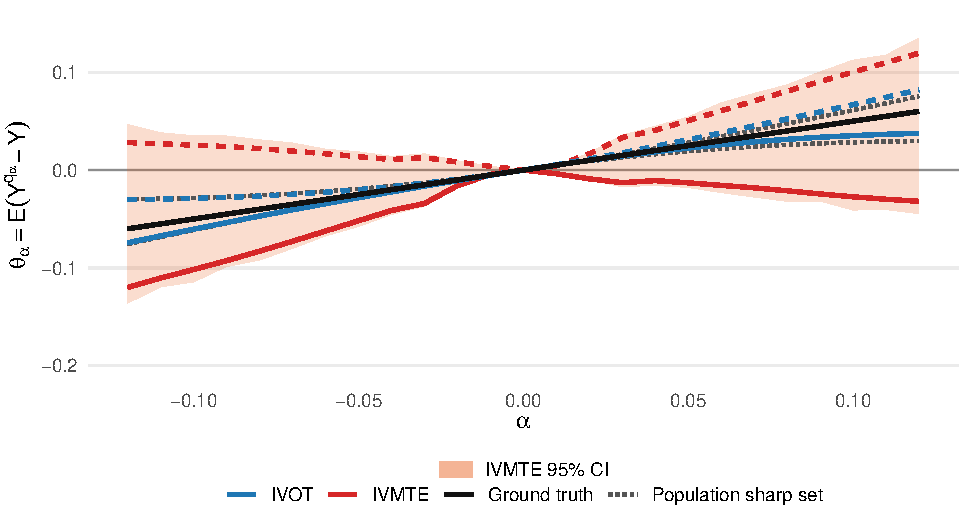
\includegraphics[width=\textwidth]{figures/prte_comparison_continuous_5000.pdf}
    \caption{Continuous-instrument IVOT and IVMTE identified sets for $\theta_\alpha = \mathbb{E}[Y^{q_\alpha}-Y]$ across policy shifts $\alpha \in [-0.12, 0.12]$ at $n=5{,}000$. Grey dotted curves: the population sharp identified set, computed in closed form. Black line: ground truth. Blue and red curves: estimated IVOT and IVMTE bounds (solid = lower, dashed = upper). Shaded ribbon: pointwise 95\% backward confidence interval for the IVMTE bounds.}
    \label{fig:synthetic_bounds}
\end{figure}

\paragraph{Discrete instrument.}
The discrete-instrument DGP uses $Z \sim \text{Bernoulli}(0.5)$ with two-point propensity score $\{0.25, 0.75\}$, to which the closed-form bounds of \cref{thm:discrete_lower_bound} apply, and a heterogeneous $\text{MTE}(u) = 0.48 + 0.18u$. The outcome support is $[0, 1.08]$ and the exact policy-effect truth is $\theta_\alpha = 0.57\alpha + 0.09\alpha^2$; both are derived in \cref{app:simulation}. \cref{fig:synthetic_bounds_discrete} shows the identified sets at $n = 5{,}000$ alongside the population sharp set. The truth falls inside the IVOT interval at all 25 grid points, and the IVOT interval is $2.4$--$3.6\times$ narrower than IVMTE throughout: at $\alpha = 0.05$ the IVOT interval is $[-0.001,\, 0.042]$ (width $0.043$) versus the IVMTE interval $[-0.051,\, 0.054]$ (width $0.105$). The gap between the two methods is enough to change the qualitative conclusion at large shifts: the estimated IVMTE identified set contains zero at every $\alpha$, whereas the estimated IVOT identified set excludes zero once $\alpha \geqslant 0.08$.

\begin{figure}[!htbp]
    \centering
    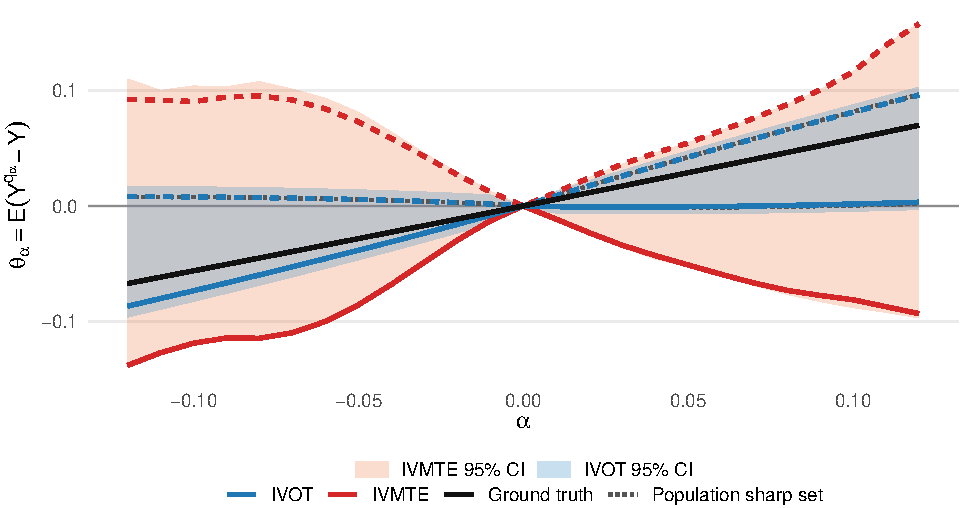
\includegraphics[width=\textwidth]{figures/prte_comparison_discrete.pdf}
    \caption{Discrete-instrument IVOT and IVMTE identified sets for $\theta_\alpha = \mathbb{E}[Y^{q_\alpha}-Y]$ across policy shifts $\alpha \in [-0.12, 0.12]$ at $n=5{,}000$. Grey dotted curves: the population sharp identified set, computed in closed form. Black line: ground truth. Blue and red curves: estimated IVOT and IVMTE bounds (solid = lower, dashed = upper). Shaded ribbons: pointwise 95\% confidence intervals for the bounds (blue = IVOT delta method, red = IVMTE backward CI).}
    \label{fig:synthetic_bounds_discrete}
\end{figure}

\paragraph{Discrete instrument with covariates.}
The third design adds five continuous covariates to a three-valued instrument, with $\text{MTE}(u,x)$ varying in both arguments, and is built so that \cref{asp:prop_gap} holds exactly with $c_{\text{gap}}=0.04$ and every component of the score is active on the reported window $\alpha\in[0.195,0.255]$, at $n=4{,}000$. As in the two designs above the comparison is against IVMTE in its nonparametric form, so the $u$-spline sieve is interacted with the covariates and the MTR is left unrestricted in shape as well as in level. \Cref{app:simulation} of \oalocation{} gives the DGP, the policy window, the comparison choices, and the numerical tables.

\cref{fig:synthetic_bounds_cov} shows the estimated IVOT interval tracking the population sharp set---closed form here up to the expectation over $X$---and containing the truth at all $11$ grid points, at $0.79$--$1.06$ times the sharp width. IVOT is narrower than IVMTE by $1.10$--$1.46\times$ at degree $3$ and $1.34$--$1.78\times$ at degree $7$, and the difference is qualitative: at $\alpha = 0.219$ the sharp set is $[0.019,\,0.134]$ and IVOT $[0.015,\,0.137]$, while IVMTE at degree $7$ returns $[-0.012,\,0.156]$. Both that interval and its pointwise 95\% backward confidence band contain zero throughout the policy-shift grid, so the moment relaxation loses the sign of the policy effect.

\begin{figure}[!htbp]
    \centering
    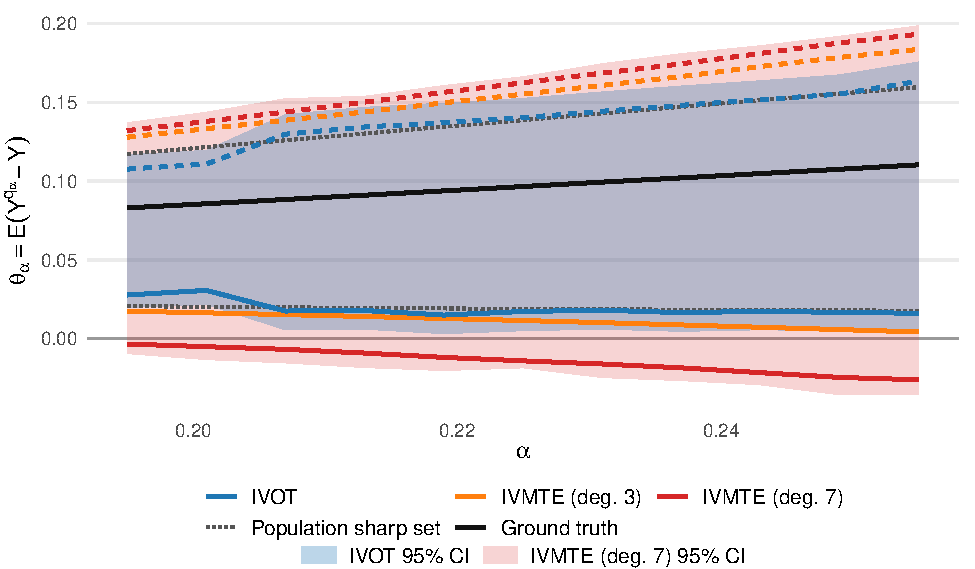
\includegraphics[width=\textwidth]{figures/prte_comparison_discrete_cov.pdf}
    \caption{Covariate design: IVOT and IVMTE identified sets for $\theta_\alpha = \mathbb{E}[Y^{q_\alpha}-Y]$ at $n=4{,}000$, with five continuous covariates and a three-valued instrument. Grey dotted curves: the population sharp identified set, computed in closed form. Black line: ground truth. Blue: IVOT (solid = lower, dashed = upper), with its pointwise 95\% interval shaded. Orange and red: IVMTE with the $u$-spline sieve interacted with the covariates, at degrees $3$ and $7$. The red shading is the pointwise 95\% backward bootstrap confidence band for the degree-$7$ IVMTE bounds. As in \cref{fig:bednet_bounds}, the richer sieve gives the wider bound.}
    \label{fig:synthetic_bounds_cov}
\end{figure}

The estimation theory of \cref{sec:est_inf} is tested separately by Monte Carlo. Over $400$ replications at each of five sample sizes from $1{,}000$ to $16{,}000$ the sampling standard deviation contracts at the parametric rate, the estimated standard errors closely match the Monte Carlo standard deviations at the larger sample sizes---their ratios rise to $1.00$ and $1.02$ for the two bounds---and the level-set recovery step returns the correct configuration in every replication once $n\geqslant8{,}000$. \Cref{app:simulation} of \oalocation{} gives the full Monte Carlo results.

\FloatBarrier
\subsection{Effect of Price Subsidies for Bed Nets}\label{sec:sim_bednet}

\paragraph{Background and setup.}
We apply our method to the bed net subsidy experiment of \citet{dupas2014subsidies}. The policy question is how the price of a bed net affects its usage, which is what a PRTE measures. For $n = 1{,}078$ Kenyan households the data contain the offered price as instrument $Z$ (17 values spanning 0--250 KSh, randomized across distribution points), purchase as treatment $W$, and one-year follow-up usage as outcome $Y$. We compare two fixed-price policies: the baseline assigns every household the reference price $z_0 = 150$ KSh, and for each $\alpha \in [0.05, 0.62]$ the alternative raises the purchase propensity from $\hat p(z_0)$ to $q_\alpha := \min(\hat{p}(z_0) + \alpha, 1)$. The target is $\text{PRTE}_\alpha = \mathbb{E}[Y^{q_\alpha} - Y^{p(z_0)}]/\alpha$; because both policies are constant in $Z$, the mean policy shift equals $\alpha$ exactly, so the denominator is the shift size rather than an estimated quantity. The baseline is the fixed-price policy $Y^{p(z_0)}$, not the observed $Y$ under randomized prices, and the grid is itself constructed from the first stage, its endpoint $\alpha_{\max}\approx 0.621$ being the estimated propensity at zero price minus the estimated baseline propensity. Because the instrument is discrete, the closed-form bounds of \cref{thm:discrete_lower_bound} apply directly to the numerator, after which we divide by $\alpha$. For IVMTE, we approximate the marginal treatment response (MTR) functions with degree-$10$ and degree-$20$ $u$-spline sieves on $[0,1]$. Full data, propensity-estimation, and policy-construction details are in \cref{app:simulation}.

\begin{figure}[!htbp]
    \centering
    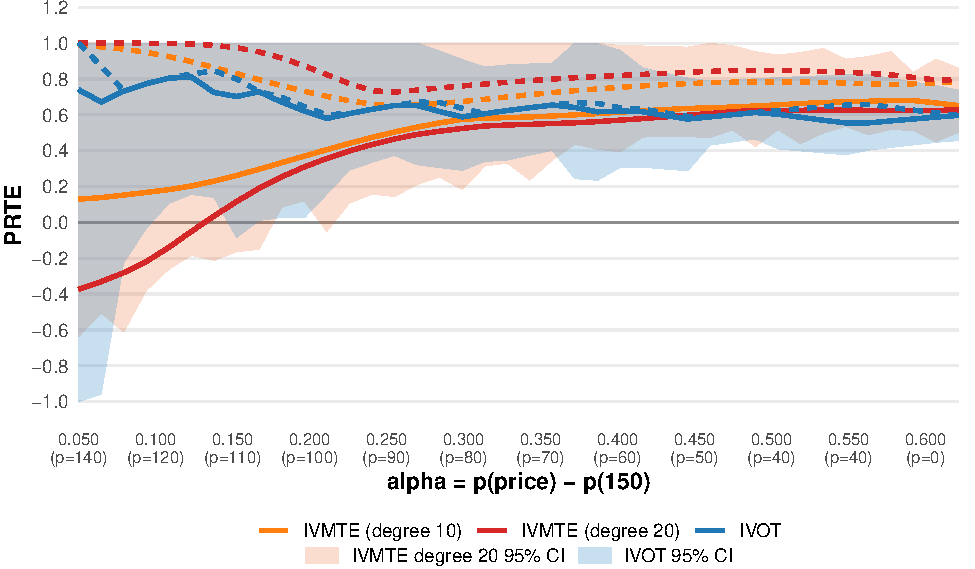
\includegraphics[width=\textwidth]{figures/prte_comparison_bednet.pdf}
    \caption{IVOT versus IVMTE identified sets for $\text{PRTE}_\alpha = \mathbb{E}[Y^{q_\alpha}-Y^{p(z_0)}]/\alpha$ on the bed net data from \citet{dupas2014subsidies}. IVMTE is shown for degree-$10$ (orange) and degree-$20$ (red) $u$-spline sieves, with solid curves the lower bounds and dashed the upper; degree~$20$ widens the bound, reflecting the more nonparametric MTR class. Shaded ribbons: pointwise 95\% confidence intervals for the estimated bounds (red = IVMTE deg.~$20$, blue = IVOT). IVOT substantially tightens the identified set and achieves near-point identification at several subsidy levels.}
    \label{fig:bednet_bounds}
\end{figure}

\paragraph{Results.}
\cref{fig:bednet_bounds} plots the IVOT and IVMTE identified sets for $\text{PRTE}_\alpha$ across subsidy levels. IVOT consistently yields a tighter identified set than IVMTE across the reported range of $\alpha$ and at both spline degrees. At the smallest subsidy ($\alpha = 0.05$), the IVOT interval is $3.3$ times narrower than IVMTE at degree $10$ and $5.3$ times narrower at degree $20$.

Both methods indicate a positive policy effect across most of the subsidy range---the IVOT lower bound is positive throughout, and the degree-$10$ IVMTE lower bound is positive for all $\alpha$, with the more conservative degree-$20$ lower bound turning positive once $\alpha \geqslant 0.14$. IVOT achieves near-point identification (width $< 0.05$) for the majority of $\alpha$ values. Those narrow identified sets do not translate one-for-one into narrower confidence intervals. \cref{app:simulation} gives more details and explanations for the wide confidence intervals.
